% \pagebreak[4]
% \hspace*{1cm}
% \pagebreak[4]
% \hspace*{1cm}
% \pagebreak[4]
%\usepackage[round,colon,authoryear]{natbib}

\chapter{Kingdom-wide discovery of bacterial intrinsic termination motifs}
\label{sec:chapterPingpong}
\ifpdf
    \graphicspath{{Chapter5/Chapter5Figs/EPS/}{Chapter5/Chapter5Figs/}}
\fi

\section{Introduction}

As discussed in the previous chapter, intrinsic termination of transcription is a fundamental cellular process in many, if not all, bacterial species. As reviewed in the previous chapter, the bulk of work on intrinsic termination has focused on canonical Rho-independent terminators (RITs), consisting of a G/C-rich hairpin structure followed by a poly-U tail. This is due to both their prevalence in model organisms such as \textit{Escherichia coli} and \textit{Bacillus subtilis}, as well as the distinctiveness of this motif making it an easy target for automated classification.

Despite this focus on canonical RITs, a number of intrinsic terminators which do not rely on a poly-U tail for termination activity are known. These include synthetic constructs derived from canonical RITs \parencite{Abe1996}, as well as naturally occurring terminators in \textit{Streptomyces} \parencite{Deng1987, Neal1991, Ingham1995} and \textit{Mycobacteria} \parencite{Unniraman2001}. Additionally, a number of ncRNA screens in Actinobacteria have described potential non-canonical RITs terminating ncRNA transcription \parencite{Swiercz2008,Miotto2012, Li2013}.  However, a more wide-spread effort at characterization of these elements has been hampered by two factors: their occurrence primarily in non-model organisms such as the Actinobacteria, and a lack of a systematic classification of these elements making it difficult to determine how wide-spread such elements are. The only study surveying potential alternative intrinsic terminators in the bacterial kingdom relied primarily on categorizing elements based on the shape of their predicted secondary structure \parencite{Unniraman2002}. However, this fails to consider the large number of very different sequences that can give rise to any particular secondary structure \parencite{Schuster1994}. It is well understood from studies of synthetic perturbations of canonical RITs that the sequence of both the hairpin structure and flanking sequence can have large, and often unexpected, effects on termination efficiency \parencite{Reynolds1992, Abe1996, Cambray2013, Chen2013}; there is no reason to think that non-canonical RITs would not exhibit a similar pattern of sequence specificity. As a result, there is a need for a robust classification of potential non-canonical RITs which considers both the sequence and structural features of these elements so that they can be systematically investigated. 

%Our view of bacterial diversity is expanding rapidly, particularly through the targeted sequencing of under-explored regions of the phylogeny \parencite{Wu2009} and recent advances in single-cell genomics enabling the sequencing of uncultivated organisms \parencite{Marcy2007, Rinke2013}, 

In the previous chapter I showed that covariance models (CMs) are able to capture sequence as well as structural features of canonical as well as putative non-canonical RITs. In this chapter I describe a method for the discovery of potential structured termination motifs across the bacterial kingdom, present an initial analysis of the elements discovered, and provide evidence for their activity through the analysis of a large collection of publicly-available RNA-seq data.

\section{Methods}

\textit{James Hadfield (University of Canterbury) ran the MCL clustering under my supervision. Paul P. Gardner (University of Canterbury) developed and ran the analysis of expression data, and assisted in manual curation of cluster alignments. Stinus Lindgreen (University of Canterbury/University of Copenhagen) processed RNA-seq data and performed mapping. I performed all other work described here. }

\subsection{Genome-wise motif discovery}
1853 embl format files containing the genomic sequence and annotations for 1639 bacteria were obtained from the EMBL European Nucleotide Archive completed bacterial genomes pages, see supplementary information for organisms and accession numbers.

Each embl file was screened independently for putative multi-copy termination motifs. For each embl file, I extracted sequences from -20 to +80 around annotated ORF\nomenclature[Z]{ORF}{Open reading frame} stop site. Each extracted sequence was screened for a lower than expected predicted MFE using RNAfold in order to screen out locally GC-rich but unstructured sequences. The sequence under consideration was shuffled 1000 times preserving dinucleotide frequencies, and a Gumbel distribution was fitted to the resulting empirical null MFE distribution using the R MASS package \parencite{Venables1994}. Sequences with a native MFE below the 95th percentile of the null distribution were discarded. The resulting set of sequences was then given as input to CMfinder \parencite{Yao2006}, which produces collections of locally-aligned structurally conserved motifs. I built a CM for each motif using Infernal 1.0.2 \parencite{Nawrocki2009}.  The resulting CMs were searched against the embl file the motif was discovered in, and were then screened on the following criteria for the collection of search hits with an E-value of less than 1: a copy number of between 100 and 3000, and a median distance of $<$10 to the nearest annotated ORF stop site. This resulted in a collection of 4359 putative termination motif CMs, each derived from a single embl file. 

\subsection{Clustering covariance models}

In order to cluster CMs, I developed an extension of MCL-based clustering \parencite{Enright2002} to generative models of sequence variation. I call the measure of CM similarity I developed for this purpose the reciprocal similarity score (RSS), defined as: \[ \left[\frac{\sum_{i=1}^{n} -\ln{(E_{x,y,i})} +  \sum_{j=1}^{n} -\ln{(E_{x,y,j})}}{2n}\right] + \ln(n) \] where $E_{x,y,i}$ is the E-value of the $i$th sequence emitted by model $x$ scored by model $y$ and for the purposes of this study $n=1000$. Briefly, for each pair of CMs 1000 sequences were emitted from each CM and reciprocally scored with the other CM. The average of the negative log-transformed E-values was calculated, then shifted to be strictly positive by adding $\ln(1000)$ to generate the RSS\nomenclature[Z]{RSS}{Reciprocal similarity score} appropriate for use with MCL. MCL was run over the resulting RSS matrix, and the 100 largest clusters, ranging in size from 332 to 6 CMs, were taken forward for further analysis.

\subsection{Building consensus covariance models}

To build covariance models which captured the diversity of sequences represented by each cluster, I searched the ten CMs with the highest sum of RSS scores in each cluster against the set of genomes which contributed motifs to the cluster. Sequences on which at least four CMs agreed on with an E-value of $<$ 1 were collected. The redundancy of the collected sequences was iteratively reduced in an alignment-free fashion using cd-hit \parencite{Li2006} with the parameters -G 0 -aL 0.1 -aS 0.3 until there were less than 2000 sequences remaining or there were no remaining sequences with $>$ 85\% nucleotide identity. Sequences were extended by 20 bases on each side to capture features which may not have been in the CMfinder-derived motifs, e.g. poorly conserved poly-U tracts. The resulting set of sequences was aligned using MAFFT Q-INS-i \parencite{Katoh2008} using McCaskill base-pairing probabilities \parencite{McCaskill1990}, and secondary structures were predicted using CentroidAlifold \parencite{Hamada2009}, again with McCaskill base-pairing probabilities. CMs were built from the resulting cluster alignments, and sequences which did not match the CM with a bitscore of at least 20 were iteratively discarded. The resulting alignments were then manually curated using RALEE \parencite{Griffiths-Jones2005}, trimming non-conserved flanking sequence and extending the predicted secondary structure where possible. Conserved stop codons were specifically trimmed, so as not to bias subsequent searches.

\subsection{Genome annotation}

The resulting cluster CMs were searched over the initial 1853 embl files. Bitscore thresholds were set for hit significance for each cluster CM using shuffled sequence. Specifically, each cluster model was also used to search a dinucleotide shuffled database of these same 1853 embl file. For each model, a Gumbel distribution was fitted to the distribution of bitscores over the shuffled database, and this null Gumbel distribution was used to compute P-values for hit significance in the native sequences. P-values were corrected for multiple hypothesis testing using the method of \textcite{Benjamini1995}, and these were used to set bitscore thresholds at specific FDRs.

\subsection{Analysis of expression data}

Data sets were downloaded from the SRA \parencite{Leinonen2011}, preferring whenever possible to start our own analyses with the raw fastq input instead of relying on previous mapping results. This was done to make the data sets comparable. After retrieving the data sets, we extracted fastq reads for further analysis. Most data sets were downloaded in SRA format. Fastq files were extracted using the command �fastqdump --split-3� from the SRA toolkit version 2.3.2-4. This creates two fastq files in the case of paired end data, and one fastq file in case of single end data. When BED files were used as the primary input, the BAM file was extracted directly using �bedToBam� from the bedtools package, version 2.17.0 \parencite{Quinlan2010}. Data sets in SOLiD format was translated to fastq using �solid2fastq� from bfast version 0.7.0a \parencite{Homer2009}. All extracted fastq files were cleaned using AdapterRemoval version 1.4 \parencite{Lindgreen2012} with the flags �--trimns --trimqualities � to remove residual adapters from the reads and to remove low quality segments and stretches of Ns in the 5� and/or 3� ends.

Most data sets were mapped using bowtie2 version 2.1 \parencite{Langmead2012}, and the output was saved in BAM format using samtools version 0.1.18 \parencite{Li2009}. In the single end case, the following command was used:
\begin{verbatim} 
bowtie2 -x <INDEX> -U <READS> |samtools view -bS - \
| samtools sort - <OUTPUT>.sorted
\end{verbatim}

In the paired end case, a similar command was used, but the number of input files was larger because 1) there are two files containing the paired reads, and 2) additional single end reads might have been produced by AdapterRemoval because some pairs were collapsed due to overlaps, or one mate pair was discarded due to e.g. low quality. For 454 data, using the above command produced few mappings to the reference genome. We therefore used bowtie2 but with relaxed parameters to accommodate the longer reads by adding the flags �--local --very-sensitive-local�. For SOLiD data, we used bfast version 0.7.0a for mapping with the following commands:
\begin{verbatim}
bfast match -f <INDEX> -A 1 -r <READS> > <OUTPUT>.bmf
bfast localalign -f <INDEX> -A 1 -m <OUTPUT>.bmf > <OUTPUT>.baf
bfast postprocess -f <INDEX> -i <OUTPUT>.baf -A 1 | samtools view -bS - \
| samtools sort - <OUTPUT>.sorted
\end{verbatim}

For each BAM-file, we generated a PLOT file containing two tab separated columns (reverse strand, forward strand) and a line per position in the genome. Each line gives information on the number of mapped reads on each strand for that particular position in the reference genome. The PLOT files were generated using the following commands from samtools version 0.1.18:
\begin{verbatim}
samtools view -F 0x10 -b <INPUT> (for reads mapped to the forward strand)
samtools view -f 0x10 -b <INPUT> (for reads mapped to the reverse strand)
\end{verbatim}
Then, the �samtools depth� command was used to get the actual depths and save them in a WIG format file, which was then transformed to PLOT file by filling out the 0-depth positions based on the length of the reference genome.

(info on plots here)

\section{Results}

\subsection{Kingdom-wide motif discovery}

The pipeline I developed for discovering putative termination motifs consisted of 3 major stages (see figure X): genome-wise motif discovery with CMfinder  \parencite{Yao2006}, clustering of motifs using a novel similarity measure and the MCL algorithm \parencite{Enright2002}, and manual curation of the resulting motif clusters.  

In the first stage I extracted sequence from -20 to +80 with respect to annotated stop sites, which were then filtered on predicted structural potential to screen for sequences with stronger structures than predicted by their dinucleotide content alone (see Methods). For each genome, I used the resulting set of sequences as input for the CMfinder alogrithm \parencite{Yao2006}. Briefly, CMfinder uses heuristic sequence search, thermodynamic and mutual information-based predictions of secondary structure, and CM-based searches within an expectation-maximization (EM\nomenclature[Z]{EM}{Expectation-maximization}) framework to iteratively discover and refine potential structured RNA motifs, returning a multiple sequence alignment and corresponding CM. CMfinder has previously been successfully used as part of pipelines for the discovery of non-coding RNAs in bacteria \parencite{Weinberg2007, Weinberg2010} and eukaryotes \parencite{Torarinsson2008a}, as well as in our previous discovery of the TRIT element \parencite{Gardner2011a}. Applying this algorithm to the filtered sequences for each genome resulted in a total of 22310 motif predictions. I searched these CMs back over the genome they were predicted from and removed from consideration motifs with very low ($<$100) or very high ($>3000$) copy number, or were not enriched with respect to gene terminal regions, leaving a set of 4359 putative termination motifs, approximately 2.5 per organism.

To reduce the complexity of this data set, I developed a method for clustering CMs. Two previous approaches to comparing CMs have been described in the literature. The first, known as CMcompare \parencite{Honer-zu-Siederdissen2010}, computes the score of a so-called `link sequence', that is a sequence with the highest value of $\min{(S_1(s), S_2(s))}$, where $S_x(s)$ is the score of sequence $s$ with respect to model $S_x$. While this has been proposed as a measure of CM specificity in the context of the Rfam database, it is unclear how accurately this single link sequence captures the overlap between the sequence spaces described by two CMs, let alone the reality of overlaps in actual biological sequence databases. A second method, proposed as part of the Evofam pipeline for automated ncRNA family discovery in eukaryotic genome alignments \parencite{Parker2011}, approximates the Kullback-Leibler divergence between two CMs, that is the similarity of the probability distributions over sequences emitted by the two CMs, using the difference in Infernal CM E-value calculations on a human reference sequence from each model's training set. In the context of the Evofam pipeline, the use of the human reference sequence is justifiable, as the study was primarily concerned with the discovery of ncRNA families present in the human genome. However, in the present case of clustering motifs across an entire domain of life, there is no obvious single sequence to use as a reference for the purposes of a comparison between every pair of CMs.

\begin{figure}[htp]
\begin{center}
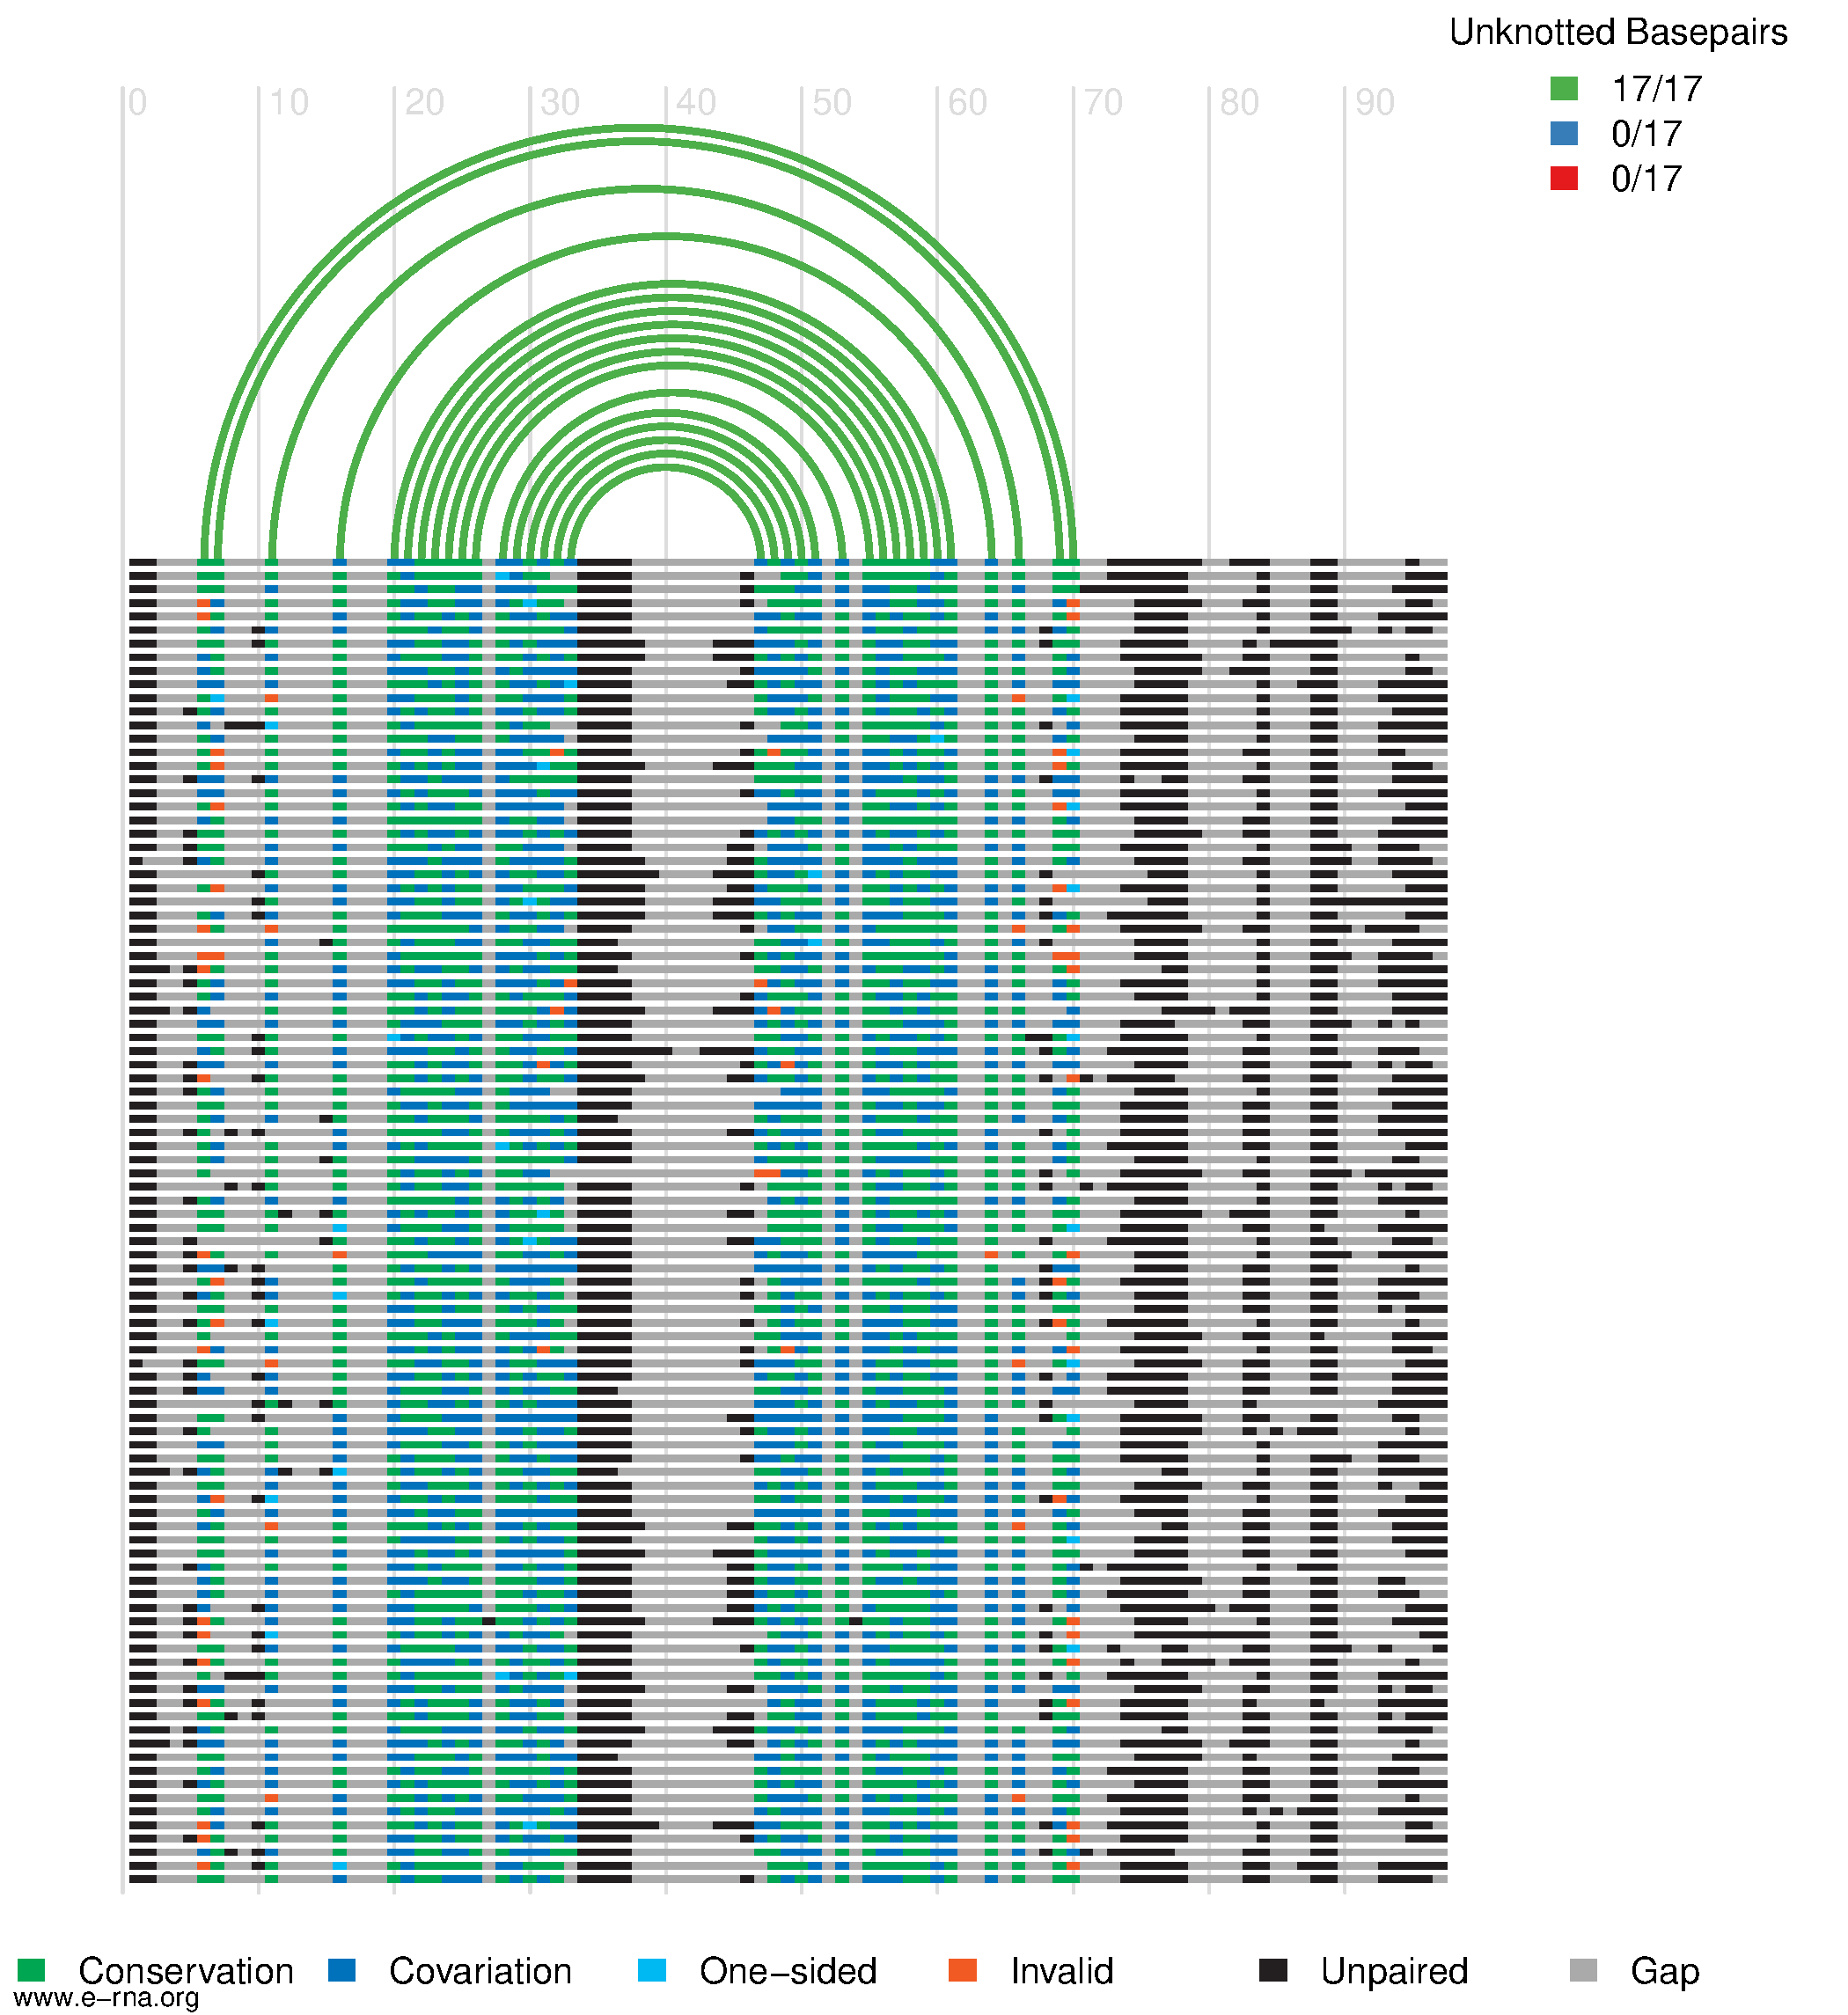
\includegraphics[width=14cm]{16_aln}
\caption[Example alignment of cluster consensus sequences]{\textbf{Example alignment of cluster consensus sequences.} Partial alignment of the consensus sequences for cluster 16, visualized using the R-CHIE webserver \parencite{Lai2012}. Green arcs represent base-pairing interactions. Nucleotides are visualized as blocks below, and are colored to highlight conservation and covariation in base-pairing relationships within the stem-loop structure.
} 
\label{fig:aln}
\end{center}
\end{figure}

I have developed a sampling based approach to measuring CM similarity. However, rather than using a single reference sequence for the purpose of comparison, I use the fact that CMs are generative models to measure the average similarity of of their respective sequence spaces. Infernal reports bitscores and E-value for each match between a CM and a given sequence region. The bitscore, ignoring the specifics of algorithm used (either CYK or Inside), is \[S = \log_2\left({\frac{P(x \mid H)}{P(x \mid R)}}\right)\] where $P(x \mid H)$ is the probability of sequence $x$ under model $H$, and $P(x \mid R)$ is the probability of $x$ under a null model $R$, generally an iid\nomenclature[Z]{iid}{Independent identically distributed (random variable)} sites model with a geometric length distribution. This score is expected to follow a Type 1 Extreme Value (or Gumbel) distribution \parencite{Karlin1990, Eddy2008}, and this empirically appears to be the case for Infernal scores \parencite{Nawrocki2007}. Hence the E-value can be calculated as \[e^{-\lambda(S - \mu)}\] where $\lambda$ and $\mu$ are fitted parameters depending on the size of the database searched and the model architecture, and normalize for these factors. So the reciprocal similarity score (RSS) I have defined: \[ RSS_{x,y} = \left[\frac{\sum_{i=1}^{n} -\ln{(E_{x,y,i})} +  \sum_{j=1}^{n} -\ln{(E_{x,y,j})}}{2n}\right] + \ln(n) \] where $E_{x,y,i}$ is the E-value of the $i$th sequence emitted by model $x$ scored by model $y$, can be understood as the average normalized bitscore of each model over the other's sequence space, and is similar in spirit to the Kullback-Leibler divergence. This measure appeared robust to the number of samples used, but this may depend in part on model complexity. As the maximal E-value in this case is $n$, $-\ln(n)$ is a theoretical lower bound on the average $-\ln{(E)}$, and the subtraction of this factor ensures that the RSS is strictly positive. It is worth noting that this measure is symmetric ignoring sampling error. Asymmetric variants may have some applications. For instance, by taking the minimum of the average bitscore under either model, one would give preference to full-length model matches in comparisons between models of various sizes due to the glocal nature of Infernal search (global with respect to the model, local with respect to sequence), and this may be preferable for determining similarity between ncRNA families. Conversely, taking the maximum may have some utility in searching for shorter motifs. In the current application, I expect all CMs to be of roughly similar sizes and symmetric measures simplify clustering. This measure should be applicable to any generative model, and so could be similarly used to cluster e.g. HMMs.

A related measure was previously used by the TRIBE-MCL algorithm to cluster protein families based on reciprocal $\log_{10}$ BLAST E-values \parencite{Enright2002}. The MCL algorithm is described in detail elsewhere \parencite{VanDongen2008}, but briefly uses simulations of random walks on a weighted graph to define clusters through an unsupervised, iterative process. Unsurprisingly, many of the clusters that were generated using MCL with RSSes appeared to be composed of CMs representing canonical RITs on visual inspection with some notable exceptions, described below. However, despite a complete lack of phylogenetic assumptions in our pipeline, we found that the majority of clusters were dominated by one or two orders, generally within the same phyla, and sometimes even a single genera. This both validates our clustering procedure and indicates that RITs, despite their small size and stereotypical composition, carry a phylogenetic signal when considered in aggregate.

To further study lineage-specific biases in terminator composition, I took the top 100 clusters, ranging in size from 332 to 6 CMs, and constructed consensus models through a semi-automated process. First, for each cluster I selected the 10 CMs with the highest sum of RSS scores with other cluster CMs (or all CMs in the case of clusters with $<$ 10 members), and searched these across all of the genomes the cluster CMs were derived from. Regions that these CMs agreed were likely to be terminator sequences were collected and aligned using MAFFT Q-INS-i \parencite{Katoh2008}, a heuristic Sankoff alignment algorithm which considers both sequence and secondary structure in alignment, and secondary structure was predicted using CentroidAlifold \parencite{Hamada2009}, and manually refined using RALEE \parencite{Griffiths-Jones2005} (see figure \ref{fig:aln}; see also Methods for detailed alignment protocol). I annotated the 1853 embl files we started with, and iteratively removed from consideration any model with at least 85\% of its sequence hits covered by another model. This left 16 putative terminator models, on which all further analysis was done.



\subsection{Lineage-specific differences in RIT utilization}

Of the 16 resulting cluster, 9 appeared to be canonical RITs on visual inspection (see figure \ref{fig:canonical}). All shared known features of canonical RITs, including a $5^\prime$ poly-A region, a G/C-rich hairpin, and a poly-U tail, but differ in stem length and base composition.

\begin{figure}[htp]
\begin{center}
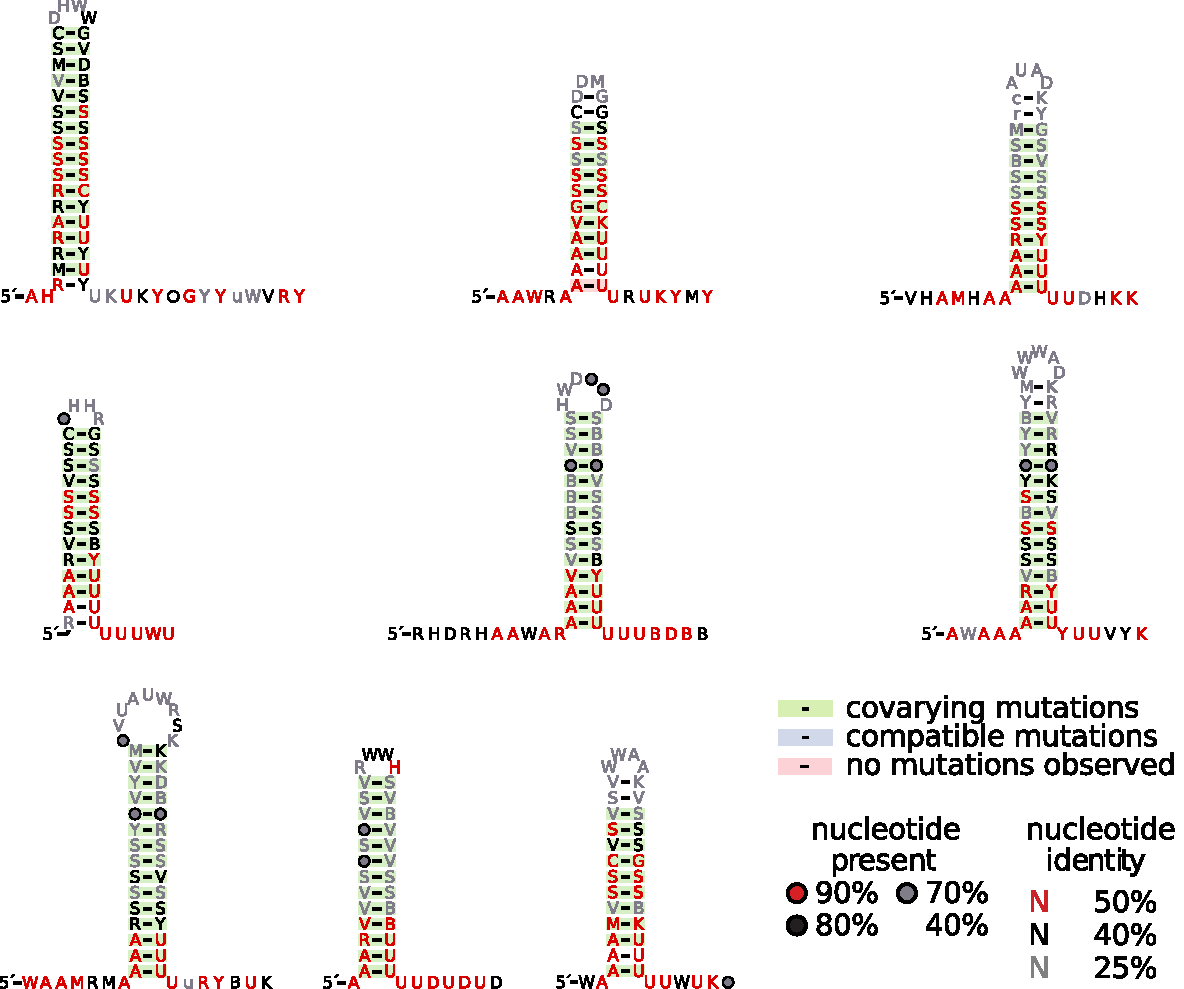
\includegraphics[width=14cm]{canonical}
\caption[Most informative sequences for nine canonical RIT clusters]{\textbf{Most informative sequence for nine canonical RIT clusters.} Each cluster consensus model was searched across all genomes and sequence hits with an FDR of 0.01 were aligned to the model. Duplicate sequences were removed and 5000 randomly sampled sequences were used to calculate the most informative sequence (MIS)\nomenclature[Z]{MIS}{Most informative sequence}, a projection of any bases with frequencies above .25 onto IUPAC characters \parencite{Freyhult2005}. Structures were drawn using R2R \parencite{Weinberg2011}. From left to right, images shown represent consensus alignments for clusters 16, 25, 29 (top row); 37, 88, 89 (middle row); 95, and 96 (bottom row).
} 
\label{fig:canonical}
\end{center}
\end{figure}

\begin{figure}[htp]
\begin{center}
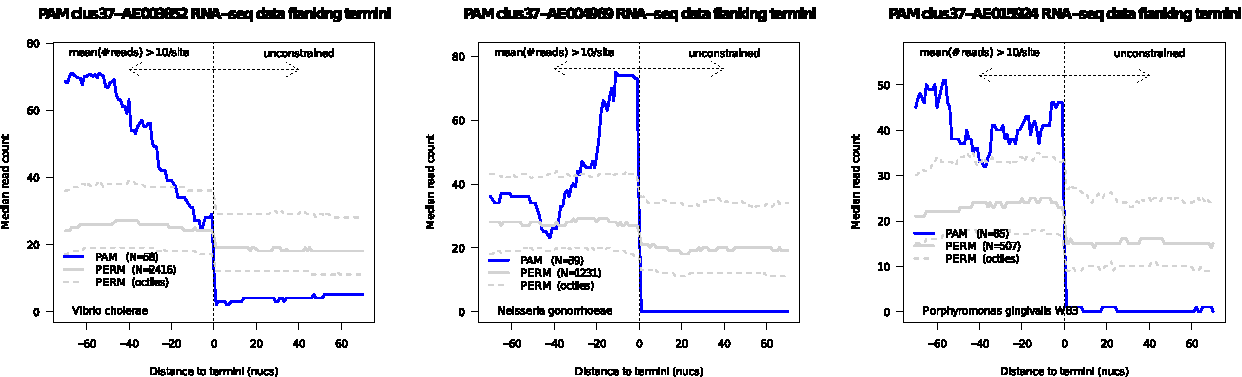
\includegraphics[width=16cm]{can_expr}
\caption[Analysis of diverse RNA-seq datasets confirm canonical terminator activity]{\textbf{Analysis of diverse RNA-seq datasets confirm canonical terminator activity.} These plots present representative analysis for putative attenuation motifs (PAM)\nomenclature[Z]{PAM}{Putative attenuation motif} by the cluster 37 canonical terminator consensus model. The median expression over PAMs with an upstream mean expression of at least 10 reads per position is plotted in blue. Random positions meeting this same constraint are plotted in grey, and the dashed grey lines provide a 75\% confidence interval for this estimate. RNA-seq data (from left to right) drawn from experiments in the $\gamma$-proteobacterium \textit{Vibrio cholerae} \parencite{Mandlik2011}, the $\beta$-proteobacterium \textit{Neisseria gonorrhoeae} \parencite{Isabella2011}, and the Bacteroidetes \textit{Porphyromonas gingivalis} \parencite{Hovik2012}.
} 
\label{fig:can_expr}
\end{center}
\end{figure}

\subsection{Non-canonical putative attenuators of transcription}

\section{Discussion}